\label{1.2.15}

\textit{The Quadric Surface in $\P^3$} (Fig. 2). Consider the surface $Q$ (a surface is a variety of dimension $2$) in $\P^3$ defined by the equation $xy - zw = 0$.

\begin{enumerate}[label = (\alph*)]
    \item Show that $Q$ is equal to the Segre embedding of $\P^1 \times \P^1$ in $\P^3$, for suitable choice of coordinates.
    
    \item Show that $Q$ contains two families of lines (a \textit{line} is a linear variety of dimension $1$) $\{L_t\}$, $\{M_t\}$, each parametrized by $t \in \P^1$, with the properties that if $L_t \neq L_u$, then $L_t \cap L_u = \emptyset$; if $M_t \neq M_u$, $M_t \cap M_u = \emptyset$, and for all $t, u$, $L_t \cap M_u = $ one point.
    
    \item Show that $Q$ contains other curves besides these lines, and deduce that the Zariski topology on $Q$ is not homeomorphic via $\psi$ to the product topology on $\P^1 \times \P^1$ (where each $\P^1$ has its Zariski topology).
\end{enumerate}

\begin{figure}
    \centering
    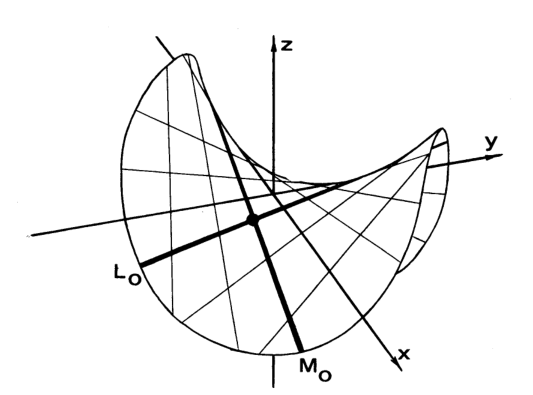
\includegraphics{Fig 02}
    \caption{The quadric surface in $\P^3$.}
    \label{Fig. 1}
\end{figure}

\begin{proof}
    
\end{proof}